\chapter{Расчёт потоков на каждой из трещин гидроразрыва} \label{ch3}

Закачиваемый в скважину расход жидкости в общем случае перераспределяется между трещинами неодинаково вследствие разного качества перфораций на трещинах и других факторов.

В данной главе будет решена задача нахождения расхода $Q_i$ на каждой $i$-ой трещине и забойного давления $p_0$ при фиксированном расходе жидкости $Q_0$ на забое скважины.

\section{Постановка задачи}
\vspace*{-5mm}

На рис. \ref{fig:flow_distribution_scheme} представлена схема перераспределения потоков между тремя трещинами гидроразрыва пласта.
На этой схеме обозначены искомые $p_0$ (забойное давление), $Q_1$, $Q_2$, $Q_3$ (расходы жидкости на трещинах), а также величины, которые важно учитывать при расчёте потоков, так как их значения существенно влияют на конечный результат.

\begin{figure}[H] 
\center
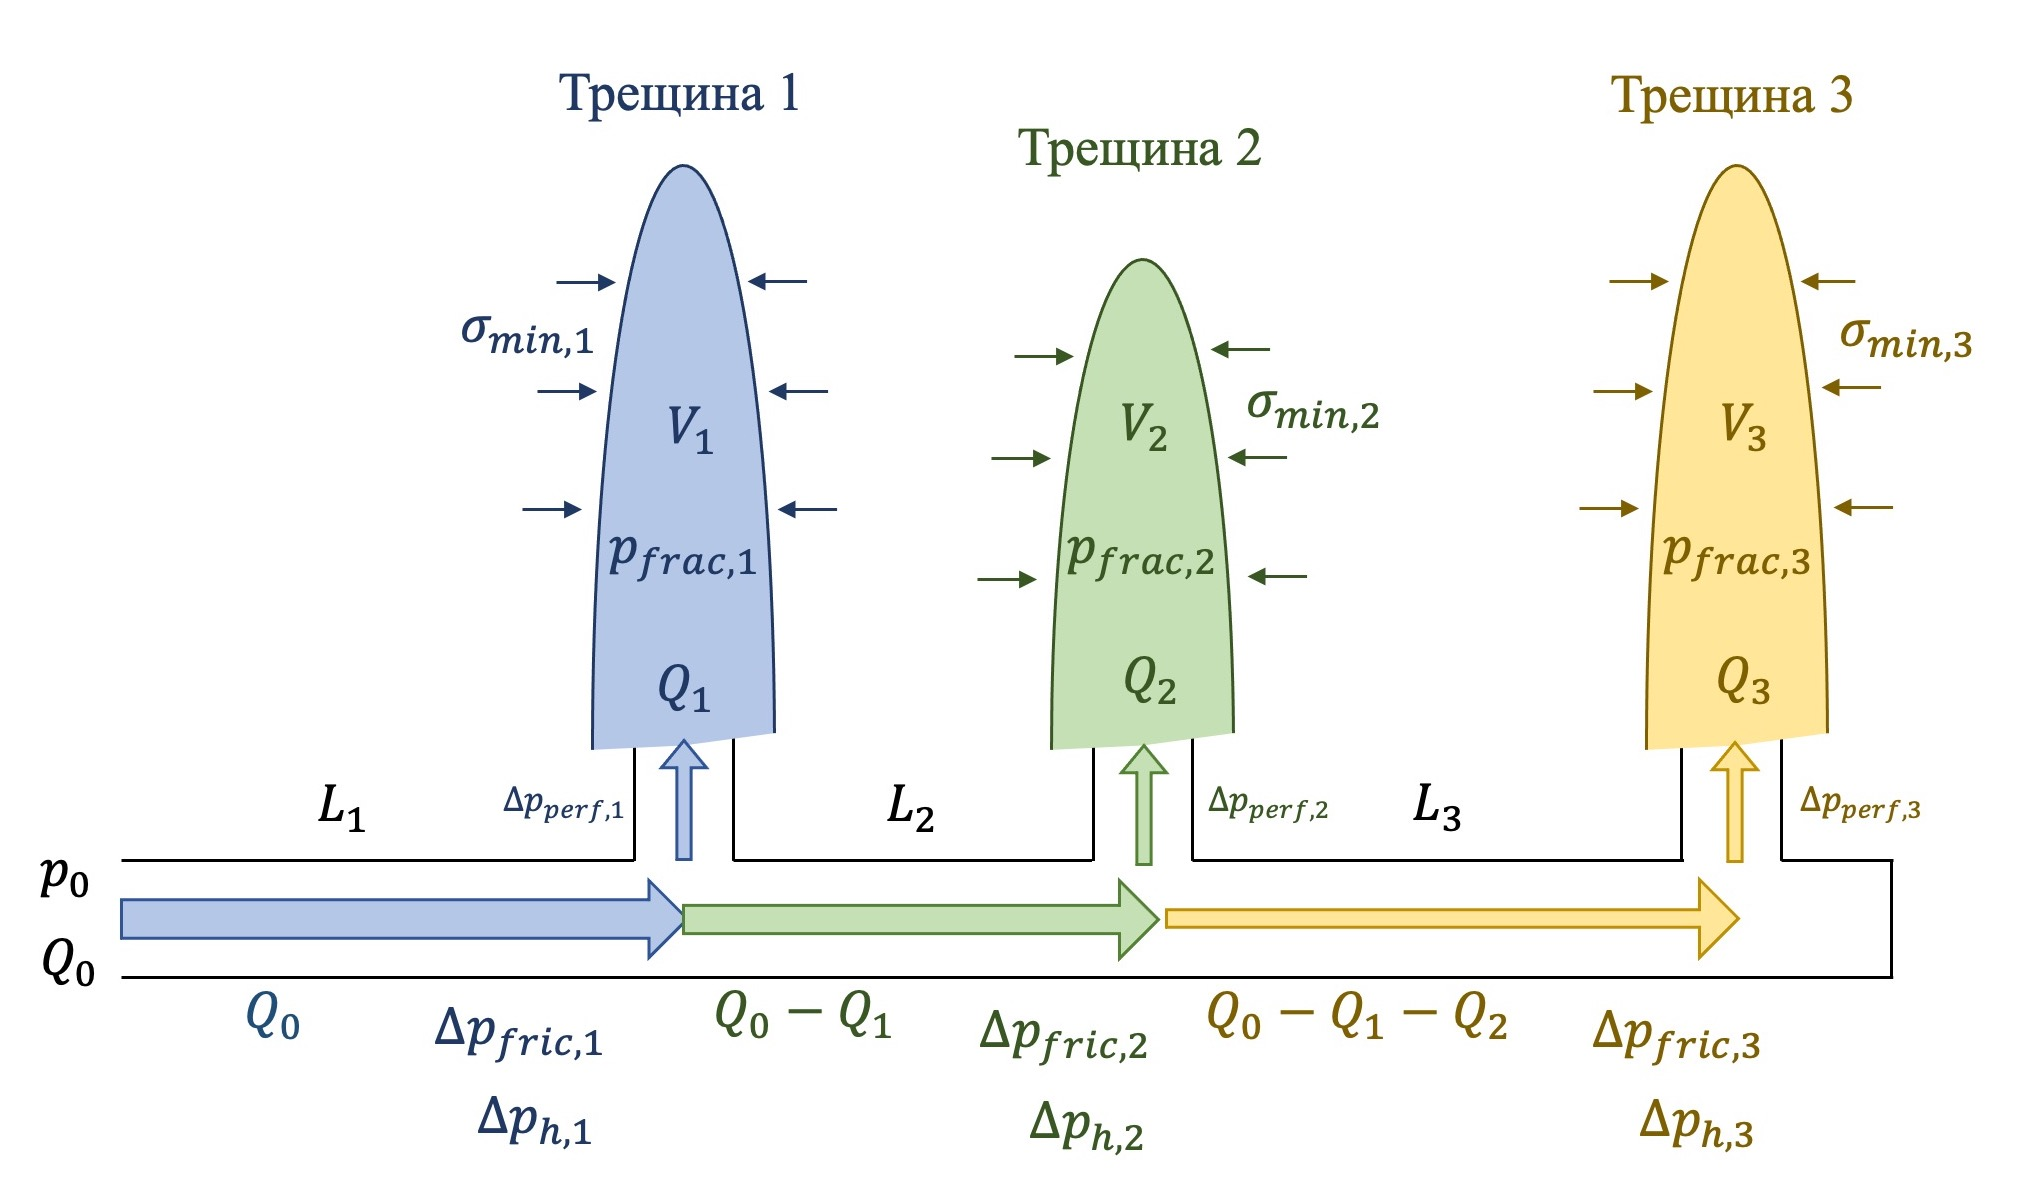
\includegraphics[width=\linewidth]{images/flow_distribution_scheme.jpg}
\caption{Схема перераспределения потоков между трещинами гидроразрыва} 
\label{fig:flow_distribution_scheme}  
\end{figure}

Согласно первому правилу Кирхгофа весь расход, который закачиваем в скважину, перераспределяется между трещинами:
\beq\label{3_1}
Q_0=\sum\limits_{i=1}^{N}Q_i,
\eeq
где $N$ -- количество трещин.

Согласно второму правилу Кирхгофа каждый из путей к каждой из трещин рассматривается независимо:
\beq\label{3_2}
p_0=\sigma_{\text{min},i}+p_{\text{net},i}+\Delta p_{\text{perf},i}-\sum_{j=1}^{i}{\Delta p_{h,j}}+\sum_{j=1}^{i}\Delta p_{\text{fric},j},
\eeq
где $\sigma_{\text{min},i}$ -- давление закрытия (минимальное напряжение в пласте) на $i$-ой трещине;\newline
$p_{\text{net},i}=p_{\text{frac},i}-\sigma_{\text{min},i}$ -- чистое давление на $i$-ой трещине (из модели трещины);\newline
$\Delta p_{\text{perf},i}$ -- падение давления вдоль перфорации $i$-ой трещины;\newline
$\Delta p_{\text{h},i}$ -- вклад гидростатического давления между $i$-ой и $(i-1)$-ой трещинами;\newline
$\Delta p_{\text{fric},i}$ -- падение давления на трение в трубе между $i$-ой и $(i-1)$-ой трещинами.

Объединяя уравнения \eqref{3_1} и \eqref{3_2}, получаем алгебраическую систему уравнений относительно $p_0$ и $Q_i$ (где $i=\overline{1, N}$).
Чтобы решить эту систему из $N+1$ уравнений с $N+1$ неизвестной, необходимо получить замыкающие соотношения на $p_{\text{net},i}$, $\Delta p_{\text{perf},i}$ и $\Delta p_{\text{fric},j}$.
Другими словами, необходимо получить зависимости этих величин от искомых величин $p_0$, $Q_i$ и других параметров, значения которых можно найти непосредственным измерением или задать при проектировании скважины.

\section{Замыкающие соотношения}
\vspace*{-5mm}

В работе \cite{kabanova_shel} получена формула для чистого давления трещины Перкинса-Керна-Нордгрена (модели PKN):
\beq\label{1_3}
p_{\text{net},i}=\sqrt{\frac{8K_{Ic,i}^2}{\pi h_{f,i}}},
\eeq
где $K_{Ic,i}$ -- трещиностойкость породы вблизи $i$-ой трещины,\newline
$h_{f,i}$ -- высота $i$-ой трещины (в случае PKN модели равна мощности продуктивной зоны).
\\

Эмпирическая формула для падения давления на перфорациях выглядит следующим образом:
\beq\label{1_4}
\Delta p_{\text{perf},i}=\frac{8\rho_s}{\pi^2 C_{d,i}^2 n_{p,i}^2 d_{p,i}^4}Q_i\left|Q_i\right|,
\eeq
где $\rho_s$ -- средняя плотность смеси;\newline
$n_{p,i}, d_{p,i}$ -- количество и диаметр перфораций;\newline\\
$C_{d,i}=\dfrac{\text{min}(d_{jet})}{d_p}$ -- безразмерный коэффициент эрозии (в случае отсутствия твёрдых частичек в потоке $C_{d,i}\in\left[0.5,0.6\right]$, а с твёрдыми частичками в потоке $C_{d,j}\in\left[0.6,0.95\right]$  из-за эрозии перфорации).
\\

Падение давления на трение на каждом интервале рассчитывается по следующей формуле:
\beq\label{1_5}
\Delta p_{\text{fric},i}=\int\limits_{x_{i-1}}^{x_i}{f\frac{\rho u_{m,i}^2}{R_i}}=\int\limits_{x_{i-1}}^{x_i}{\frac{\rho(c(t,s))\cdot f(Re)\cdot \left(Q_0-\sum\limits_{j=1}^{i-1}{Q_j}\right)^{\!2}}{R_i(s)S_i^2(s)}}ds,
\eeq
где $f=\dfrac{\tau}{\rho u_{m,i}^2/2}$ -- коэффициент трения Фаннинга;\newline\\
$\rho(c(t,s))$ -- плотность смеси, которая зависит от динамически меняющейся концентрации проппанта;\newline\\
$u_{m,i}=\dfrac{Q_0-\sum\limits_{j=1}^{i-1}{Q_j}}{S_i}$ -- средняя скорость на рассматриваемом участке трубы;\newline\\
$S_i$ -- площадь сечения рассматриваемого участка трубы;\newline
$R_i$ -- радиус рассматриваемого участка трубы;\newline
$Re$ -- число Рейнольдса.

Подставляя выражения \eqref{1_3}, \eqref{1_4} и \eqref{1_5}, в законы Кирхгофа \eqref{3_1} и \eqref{3_2}, получаем систему нелинейных алгебраических уравнений, которая может быть решена численно с помощью метода Ньютона.

В следующем разделе будут рассмотрены различные модели трещин гидроразрыва и их ограничения.
Будет выбрана наиболее подходящая модель для описания роста трещин автоГРП.

\section{Описание численного алгоритма решения}

\section{Результаты}
